%%%
% Universidade Estadual do Oeste do Paraná - Unioeste
% Centro de Ciências Exatas e Tecnológicas
% Curso de Bacharelado em Ciência da Computação
% Conteúdo: Arquivo principal para a compilação do TCC
% Obs.: Para maiores personalizações, veja o arquivo "unioeste.sty"
%%%
\documentclass[12pt, oneside, a4paper, brazil]{book}

% ---
% Tratamento de acentos / charset
% ---
\usepackage[T1]{fontenc}
% Em caso de problemas na compilação, tente alternar os packages abaixo:
% \usepackage[latin1]{inputenc}
\usepackage[utf8]{inputenc}
% ---

\usepackage{unioeste}

% ---
% Atalhos p/ capa, rosto, aprovacao
% ---
\newcommand{\autor}{Leonardo Pereira Merlin}
\newcommand{\ferramenta}{E4J} % nome da ferramenta
\newcommand{\titulo}{\ferramenta: Editor \emph{i}* para JGOOSE}
% Datas
\newcommand{\ano}{2013}
\newcommand{\datalonga}{28 de maio de \ano}
% Banca
\newcommand{\orientador}{Victor Francisco Araya Santander}
\newcommand{\membroA}{Ivonei Freitas da Silva}
\newcommand{\membroB}{Elder Elisandro Schemberger}

% ---
% document
% ---
\begin{document}

% numeracao em romanos para paginas iniciais (capa, agradecimentos, etc)
\pagestyle{empty}
\pagenumbering{roman}

% paginas iniciais
\begin{wrapfigure}[4]{i}{0cm}
	\centering
	
\includegraphics[width = 3.13cm, height = 2.19cm]{Figuras/Simbolo.jpg}
\end{wrapfigure}
\fontsize{13}{13}
\noindent
\textbf{Unioeste - Universidade Estadual do Oeste do Paran\'{a}}\\
\fontsize{11}{11}
CENTRO DE CI\^{E}NCIAS EXATAS E TECNOL\'{O}GICAS\\
Colegiado de Ci\^{e}ncia da Computa\c{c}\~{a}o\\
\textbf{\textit{Curso de Bacharelado em Ci\^{e}ncia da Computa\c{c}\~{a}o}}
\vspace{9cm}
\begin{center}
\fontsize{13}{13}
\textbf{\titulo}\\
% \textbf{Desenvolvendo e Integrando um Editor i* ao JGOOSE}\\
\vspace{0.3cm}
\textit{\autor}\\
\vspace{9cm}
\textbf{CASCAVEL}\\
\textbf{\ano}
\end{center}

% Universidade Estadual do Oeste do Paran\'{a} - UNIOESTE
% Centro de Ci\^{e}ncias Exatas e Tecnol\'{o}gicas
% Curso de Bacharelado em Inform\'{a}tica
% Arquivo: Rosto.Tex
% Conte\'{u}do: Folha de Rosto para o Arquivo do TCC.

%%%%%%%%%%%%%%%%%%%%%%%%%%%%%%%%%%%%%%%%%%%%%%%%%%%%%%%%%%%%%%%%%%%%%
%%%
%%% Folha de Rosto
%%%
%%%%%%%%%%%%%%%%%%%%%%%%%%%%%%%%%%%%%%%%%%%%%%%%%%%%%%%%%%%%%%%%%%%%%

\fontsize{12}{12}
\begin{center}
\textbf{Leonardo Pereira Merlin}\\
\vspace{8cm}
\fontsize{14}{14}
\textbf{E4J: Editor i* para JGOOSE}\\
%\textbf{Desenvolvendo e Integrando um Editor i* ao JGOOSE}\\
\vspace{2cm}
\end{center}
\fontsize{12}{12}

\begin{flushright}
\begin{minipage}[10cm] {8.5cm}
Monografia apresentada como requisito parcial para obten\c{c}\~{a}o do grau de Bacharel em Ci\^{e}ncia da Computa\c{c}\~{a}o, do Centro de Ci\^{e}ncias Exatas e Tecnol\'{o}gicas da Universidade Estadual do Oeste do Paran\'{a} - Campus de Cascavel

\vspace{1.5cm}
\noindent
Orientador: Prof. Victor Francisco Araya Santander
\end{minipage}
\end{flushright}

\vspace{5.5cm}
\begin{center}
CASCAVEL\\
2013
\end{center}

%%%%%%%%%%%%%%%%%%%%%%%%%%%%%%%%%%%%%%%%%%%%%%%%%%%%%%%%%%%%%%%%%%%%%
%%% folha de aprova\c{c}\~{a}o
%%%%%%%%%%%%%%%%%%%%%%%%%%%%%%%%%%%%%%%%%%%%%%%%%%%%%%%%%%%%%%%%%%%%%

\begin{center}
\fontsize{12}{12}
\textbf{Leonardo Pereira Merlin}\\
\vspace{3cm}
\fontsize{14}{14}
\textbf{Desenvolvendo e Integrando um Editor i* ao JGOOSE}\\
\vspace{3cm}
\fontsize{10}{10}
Monografia apresentada como requisito parcial para obten\c{c}\~{a}o do T\'{\i}tulo de Bacharel em Ci\^{e}ncia da Computa\c{c}\~{a}o, pela Universidade Estadual do Oeste do Paran\'{a}, Campus de Cascavel, aprovada pela Comiss\~{a}o formada pelos professores:\\
\vspace{2cm}
\begin{flushright}
\begin{minipage}[10cm] {8.5cm}
\begin{center}
\rule{6cm}{0.01mm}\\
Prof. Victor Francisco Araya Santander\\
Colegiado de Ci\^{e}ncia da Computa\c{c}\~{a}o, UNIOESTE\\
\vspace{1cm}
\rule{6cm}{0.01mm}\\
Prof. Ivonei Freitas da Silva\\
Colegiado de Ci\^{e}ncia da Computa\c{c}\~{a}o, UNIOESTE\\
\vspace{1cm}
\rule{6cm}{0.01mm}\\
Prof. Elder Elisandro Schemberger\\
Colegiado de Ci\^{e}ncia da Computa\c{c}\~{a}o, UNIOESTE\\
\end{center}
\end{minipage}
\end{flushright}
\vspace{3.5cm}
Cascavel, 31 de maio de 2013
\end{center} 

\oneandhalfspacing

%Itens opcionais
%%%%%%%%%%%%%%%%%%%%%%%%%%%%%%%%%%%%%%%%%%%%%%%%%%%%%%%%%%%%%%%%%%%%%
%%%
%%% Dedicat\'{o}ria
%%%
%%%%%%%%%%%%%%%%%%%%%%%%%%%%%%%%%%%%%%%%%%%%%%%%%%%%%%%%%%%%%%%%%%%%%

\begin{center}
\fontsize{14}{14}
%\textbf{DEDICAT\'{O}RIA}
\end{center}

\vspace{10cm}

\begin{flushright}
  \begin{minipage}[10cm] {8.5cm}
  \emph {Oscar Jos\'{e} Merlin J\'{u}nior, dedico este trabalho a voc\^{e}, meu irm\~{a}o e minha refer\^{e}ncia. }
  \end{minipage}
\end{flushright}

\begin{center}
\fontsize{14}{14}
%\textbf{EP\'{I}GRAFE}
\end{center}

\vspace{10cm}

\begin{flushright}
\begin{minipage}[10cm] {8.5cm}

  \emph {"Se voc\^{e} pensa que pode ou se pensa que n\~{a}o pode, de qualquer forma voc\^{e} est\'{a} certo."
	\\Henry Ford}

\end{minipage}
\end{flushright}

%%%%%%%%%%%%%%%%%%%%%%%%%%%%%%%%%%%%%%%%%%%%%%%%%%%%%%%%%%%%%%%%%%%%%
%%%
%%% Folha de Agradecimentos
%%%
%%%%%%%%%%%%%%%%%%%%%%%%%%%%%%%%%%%%%%%%%%%%%%%%%%%%%%%%%%%%%%%%%%%%%

\begin{center}
\fontsize{14}{14}
\textbf{AGRADECIMENTOS}
\end{center}
\vspace{2cm}

Em primeiro lugar, eu gostaria de agradecer ao meu orientador, professor Victor Francisco Araya Santander, pelos conselhos, al\'{e}m do apoio, disponibilidade e interesse no meu trabalho.
Apresentou-me oportunidades que eu jamais acreditava que teria novamente.
E, al\'{e}m de acreditar nos resultados, sempre me inspirou coragem e \^{a}nimo para cumprir meus objetivos.

Tamb\'{e}m gostaria de agradecer aos outros membros da banca examinadora, os professores Ivonei Freitas da Silva e Elder Elisandro Schemberger. Obrigado por analisar e avaliar cuidadosamente o meu trabalho. Durante as apresenta\c{c}\~{o}es, contribuiram significativamente com questionamentos e sugest\~{o}es, de fato, relevantes. E n\~{a}o distante desses, meus sinceros agradecimentos a todos os acad\^{e}micos integrantes do grupo de estudo do Laborat\'{o}rio de Engenharia de Software (LES). Dentre esses, um agradecimento especial aos companheiros Diego Peliser, Leonardo Zanotto Baggio e Rodrigo Trage. Obrigado pelas apresenta\c{c}\~{o}es e discuss\~{o}es sobre temas de destaque na \'{a}rea de Engenharia de Software. Espero poder retribuir e contribuir para com o grupo.

Quanto aos colegas de moradia, Lucas In\'{a}cio, Bruno Belorte, Marcos Schmitt, Nicolas Zaro e Julian Ruiz Diaz, obrigado pela toler\^{a}ncia e bons momentos.

N\~{a}o posso deixar de agradecer os amigos Fernando Dal Bello, Amadeu Paix\~{a}o e Felipe Carminati pelas experi\^{e}ncias profissionais, oportunidades de um trabalho em equipe bem realizado e um amadurecimento pessoal memor\'{a}vel (nada que uma boa trilha sonora n\~{a}o resolva). Em especial, agrade\c{c}o ao Carlos Henrique de Fran\c{c}a, que me ajudou a esclarecer e agu\c{c}ar minhas pesquisas, al\'{e}m das cr\'{\i}ticas em numerosas vers\~{o}es de documentos t\'{e}cnicos.

% Os grandes amigos "imagin\'{a}rios", Victor Hudo e Roberto Pacheco Leal da Silva, que sempre me incentivaram das mais variadas maneiras. Esse Brasil \'{e} pequeno de mais para nos separar das \'{o}timas aventuras.

A minha fam\'{\i}lia, pelos conselhos (n\~{a}o ignorados), pelo aux\'{\i}lio e suporte de diversas maneiras. E, Lah (Larissa Torquato de Oliveira e fam\'{\i}lia), este lugar tamb\'{e}m \'{e} de voc\^{e}s.

A minha companheira, Jamile Merlin, por participar de mais esta fase da minha vida.

\`{A} todos, meu sincero agradecimento!

% Agradecer Portal da CAPES? pelos ARTIGOS - GOVERNO?


% Volta a numeração arábica
\pagestyle{plain}
%%%%%%%%%%%%%%%%%%%%%%%%%%%%%%%%%%%%%%%%%%%%%%%%%%%%%%%%%%%%%%%%%%%%%
%%%
%%% Lista de Figuras
%%% Lista de Tabelas
%%% Lista de S\'{\i}mbolos
%%% Sum\'{a}rio
%%%
%%%%%%%%%%%%%%%%%%%%%%%%%%%%%%%%%%%%%%%%%%%%%%%%%%%%%%%%%%%%%%%%%%%%%

\pagebreak
\addcontentsline{toc}{chapter}{Lista de Figuras}
\listoffigures

%\pagebreak
%\addcontentsline{toc}{chapter}{Lista de Tabelas}
%\listoftables

\pagebreak
\addcontentsline{toc}{chapter}{Lista de Abreviaturas e Siglas}
\chapter*{Lista de Abreviaturas e Siglas}
\begin{tabular}{ll}
	API			& \textit{Application Programming Interface}\\
	CASE		& \textit{Computer-Aided Software Engineering}\\
	DFD			& Diagrama de Fluxo de Dados\\
    EMF         & \textit{Eclipse Modelling Framework}\\
    ER          & Engenharia de Requisitos\\
    ES          & Engenharia de Software\\
    GOOSE       & \textit{Goal into Object Oriented Standard Extension}\\
    GUI         & \textit{Graphical User Interface}\\
	IDE			& \textit{Integrated Development Environment}\\
	ITU			& \textit{International Telecommunication Union}\\
	JGOOSE		& \textit{Java Goal into Object Oriented Standard Extension}\\
    OME         & \textit{Organization Modelling Environment}\\
    ORM         & \textit{Object-Relational Mapping}\\
    POM         & \textit{Project Object Model}\\
	POO			& Paradigma Orientado a Objetos\\
	% SGBD		& Sistema Gerenciador de Banco de Dados\\
    % SO        & Sistemas Operacionais\\
    SD          & Modelo de Dependências Estratégicas\\
    SR          & Modelo de Razões Estratégicas\\
	UML			& \textit{Unified Modeling Language}\\
	XMI			& \textit{Xml Metadata Interchange}\\
	XML			& \textit{eXtensible Markup Language}\\
	% UNIOESTE 	& Universidade Estadual do Oeste do Paraná\\
\end{tabular}

%\pagebreak
%\addcontentsline{toc}{chapter}{Lista de S\'{\i}mbolos}
%\chapter*{Lista de S\'{\i}mbolos}
%\begin{tabular}{ll}

%%
%% Humanos
%%

% Compartimentos
%	$Sh$ & Total de humanos no estado suscet\'{\i}vel\\
%	$Eh$ & Total de humanos no estado exposto\\
%	$Ih$ & Total de humanos no estado infectante\\
%	$Rh$ & Total de humanos no estado recuperado e renovado\\
		

%\end{tabular}
\pagebreak
\addcontentsline{toc}{chapter}{Sum\'{a}rio}
\tableofcontents
 % Listas(Figuras,Tabelas,Smbols) e Sumrio
\chapter*{Resumo}
\addcontentsline{toc}{chapter}{Resumo}
\noindent

Em discussões pertinentes à engenharia de requisitos, tanto em âmbito
acadêmico quanto industrial, ressalta-se que um dos principais desafios da área
consiste na integração de modelos organizacionais às demais etapas do processo
de engenharia de requisitos.

Alguns trabalhos relacionados já apresentaram técnicas para a realização dessa integração. Nesse sentido, em 2006 foi
desenvolvida uma solução computacional denominada JGOOSE (do inglês Java Goal Into Object Oriented Standard Extension),
uma ferramenta de auxílio a engenharia de requisitos que proporciona a automatização do 
mapeamento de modelos e diagramas do framework i* para casos de uso UML.

Apesar das atualizações e melhorias realizada por outros pesquisadores e membros
do grupo do Laboratório de Engenharia de Software (LES) da Universidade Estadual do Oeste do Paraná (UNIOESTE - Campus Cascavel/PR),
a ferramenta ainda possui uma dependência crítica em relação à elaboração dos dados de entrada.
Nas condições atuais é necessário instalar alguma ferramenta específica para produzir o arquivo no formato TELOS.

Desta forma,
	este trabalho consiste no projeto e desenvolvimento de um editor gráfico de modelos organizacionais i* integrado à ferramenta JGOOSE, visando melhorar suas funcionalidades e diminuir a necessidade de outros softwares para este fim.
	Uma característica importante desse novo editor é o suporte à especificação iStarML - um formato de arquivo baseado em XML para representação e intercâmbio de modelos i*.


\vspace{1cm}

\noindent
\textbf{Palavras-chave: } E4J, JGOOSE, iStarML, Modelagem Organizacional, Engenharia de Requisitos.

%=======================================================================
% Definir um estilo para páginas completas (cabealho + rodapé)
\pagestyle{plain}

% Marca de captulo do tipo "2. Blblbl..." no cabealho
\renewcommand{\chaptermark}[1]{\markboth{\thechapter.\ {#1}}{}}

% Para aumentar o tamanho da caixa para o cabealho
\addtolength{\headheight}{\baselineskip}

% Definindo o contedo do cabealho...
\fancyhf{}
\fancyhead[LO,LE]{\nouppercase{\textsf{\leftmark}}}
\fancyhead[RO,RE]{\thepage}


\fancypagestyle{plain}{
	% Para garantir que a primeira página de cada capítulo
	% não contenha nada (paginação, cabeçalho, rodapé)
	\fancyhf{} % clear all six fields
	\renewcommand{\headrulewidth}{0pt}
}

%=======================================================
% Capitulos sao numerados arabicamente
\pagenumbering{arabic}

\oneandhalfspacing
% Inclusão dos capítulos
% Capítulo 1
\chapter{Introdução}
    \label{cap:introducao}
        % intro
            Este primeiro capítulo tem como objetivo a apresentação geral do trabalho.
            É realizada a contextualização e delimitação da pesquisa ao escopo da Engenharia de Software,
            bem como
            são destacados os principais objetivos da proposta.
        % topicos
            % contexto <#ID_883627655>
                Apresenta-se inicialmente,
                na seção \ref{cap:introducao:sec:contexto},
                o contexto sobre as ferramentas de modelagem organizacional e suas contribuições na área da Engenharia de Requisitos, destacando a influência dessas ferramentas no desenvolvimento de produtos de qualidade.
            % motivacao <#ID_828369918>
                Na seção \ref{cap:introducao:sec:motivacao}, são apresentadas as principais influências e motivações para a realização do trabalho.
            % proposta <#ID_1542036198>
                Em seguida,
                na seção \ref{cap:introducao:sec:proposta},
                é apresentada a proposta sob uma visão geral e os objetivos norteadores da pesquisa.
            % contribuicoes <#ID_1701692394>
                Na seção \ref{cap:introducao:sec:contribuicoes},
                 descreve-se as contribuições esperadas após a finalização deste trabalho.
            % organizacao <#ID_1115413878>
                Por fim,
                 na seção \ref{cap:introducao:sec:organizacao},
                é apresentada a estrutura geral e a organização do restante desta monografia.
    \section{Contexto}
        \label{cap:introducao:sec:contexto}
        % backlink - resumo <#ID_1358290520>
        % Contexto - Ferramentas
            Muitas são as opções de ferramentas e técnincas para engenheiros de requisitos
            que visam auxiliar na construção de modelos organizacionais i*
                % Site i* Wiki
                \cite{site2013iwiki}
                %A Comparative Analysis of i*Agent-Oriented Modelling Techniques
                \cite{grau2006comparative}.
            Essas ferramentas, normalmente do tipo CASE (do inglês, \emph{Computer-Aided Software Engineer})
                \footnote{Ferramentas CASE, é toda e qualquer ferramenta baseada em computador que auxilie nas atividades de desenvolvimento de software.}
                 \cite{case1985computer}
            têm por objetivo tanto o aumento da produtividade nos processos da Engenharia de Software quanto a melhoria da qualidade final dos softwares.
        % Contexto - E.R.

            A área de Engenharia de Requisitos (ER),
            subárea da Engenharia de Software e responsável por diversas atividades que abrangem os processos de análise, elicitação, especificação, avaliação, ajuste, documentação e evolução dos requisitos de um sistema computacional,
            é vista como uma das mais críticas para o sucesso e qualidade de um projeto de software
                %Engnharia de Requisitos
                \cite{sommerville1998requirements}.
            Pesquisas pertinentes à ER, tanto em âmbito acadêmico quanto industrial,
            apontam a falta de um entendimento adequado da organização por parte dos responsáveis pela elaboração do documento de requisitos
            como sendo uma das principais falhas no processo de especificação dos requisitos
                % refs
                    \cite{van2000requirements}.
        % Contexto - solução: modelagem organizacional

            % intro
                Para tentar diminuir os problemas relacionados as fases iniciais do projeto,
                pesquisas recentes mostram que a comunidade tem buscado estabelecer e utilizar padrões de técnicas, métodos e ferramentas para tratar especificamente
                da fase inicial de desenvolvimento de software
                    % ref
                        % A Literature Survey on International Standards for Systems Requirements Engineering
                        \cite{schneider2013literature}.
                Pensando nisso,
                têm-se investido esforços no processo de modelagem organizacional.
            % conceito
                Este tipo de modelagem
                visa prover recursos que permitam modelar
                as intenções, relacionamentos e motivações
                entre membros de uma organização
                % refs
                    % A Conceptual Basis for Organizational Modelling
                    % mason1997conceptual <workspace:/../../../../E:/unioeste/BCC/TCC-2013/referencias/mason1997conceptual.pdf>
                    \cite{mason1997conceptual}.
            % modelagem i*
                Dentre as técnicas de modelagem organizacional,
                destaca-se a i*,
                proposto por
                    \cite{yu1993modeling},
                uma técnica que utiliza a orientação a agentes
                    \cite{yu2001agent}
                %
                    com enfoque
                    tanto nos desejos e intenções desses agentes, quanto suas dependências
                    %refs
                        \cite{site2013iwiki}
                        \cite{yu1997towards}.
                Mais detalhes sobre esta técnica e suas variações serão discutidos no capítulo
                \ref{cap:framework}.
        % Contexto - Mapeamento Modelagem / UseCase UML

            Pensando em auxiliar no processo de desenvolvimento de software,
            alguns trabalhos foram propostos com o intuito de realizar o mapeamento
            de modelos do \emph{framework} i*
            para diagramas da UML (do inglês \emph{Unified   Modeling   Language}).
            Dentre esses trabalhos, destaca-se o trabalho de Santander \cite{santander2002integrando},
            que propõe a derivação em casos de uso UML a partir de modelos do \emph{framework} i*.
        % Contexto - JGOOSE
            % intro
                Para apoiar esse processo de derivação,
                foi desenvolvida a ferramenta JGOOSE (Java Goal Into Object Oriented Standard Extension).
                Inicialmente apresentada como GOOSE em
                    \cite{pedroza2004ferramentas}
                    e
                    \cite{brischke2005desenvolvimento},
                em seguida, melhorada e apresentada como JGOOSE por
                    \cite{vicente2009},
                passou também por melhorias com
                    \cite{brischke2012melhorando}
                e, atualmente,
                está sendo aprimorada por
                    \cite{peliser2013aprimorando}.
                Consiste numa ferramenta que, seguindo algumas diretrizes e passos, mapeia de forma automática os diagramas i* para casos de uso UML.
                Ou seja, dado como entrada os modelos i*, no formato de arquivo TELOS
                    \cite{mylopoulos1990telos}
                    \cite{koubarakis1989telos},
                a ferramenta consegue gerar conforme o template proposto em
                    %ref
                    \cite{cockburn2001writing}
                os casos de uso UML com um bom nível de detalhamento.
            % problema 1 - dependência

                Porém, a ferramenta JGOOSE ainda não possui funcionalidades para a produção dos arquivos de entrada da ferramenta.
                Ainda existe a dependência da ferramenta OME ou, mais especificamente, ao formato de arquivo TELOS.
            % solução 1 - editor integrado
                Nesse contexto, percebe-se a necessidade de se desenvolver um editor de modelos i* integrado à ferramenta JGOOSE,
            % solução 2 - iStarML
                bem como implementar o suporte à especificação do formato de arquivo iStarML
                    % referenciar a proposta inicial do istarml
                    \cite{cares2007istarml},
                uma formato em XML
                para representação de modelos i*
                com o propósito de servir como um intercâmbio entre os outros meta-modelos existentes
                    \cite{colomer2011model}.
    \section{Motivação}
        \label{cap:introducao:sec:motivacao}
        % backlink - resumo <#ID_1432075869>
        % O que me motivou?
            % Motivo, Causa, Razão ou Circunstância
            % É uma área em crescimento e destaque. Muito esforço já se investiu em ferramentas CASE.
            % PQ é valido o esforço para aprimorar a ferramenta?
        % Motivacional 0 - Resolver algum dos Problemas mencionados no contexto
            % JGOOSE não possui um editor i*
            % Dependência de outras ferramentas p/ ler Telos
            % iStarML
        % Motivacional 1 - Ajudar a comunidade
            A área de Engenharia de Requisitos está em crescimento e destaque
            por impactar de forma tão significativa nos resultados finais de um projeto de software.
            Desta forma,
            é valido o investimento de esforços para a melhoria de métodos, técnicas ou ferramentas que auxiliem os profissionais da área a aprimorar seu trabalho de forma eficiente.
            % framework i*
                % padrão internacional
                    O i* é a base da GRL (\emph{Goal-oriented Requirements Language} ou Linguagem de Requisitos Orientada a Objetivos),
                    que junto à UCM
                        \footnote{UCM - \emph{Use Case Maps} , em português: "Mapas de Caso de Uso". Uma técnica de engenharia de software baseada em cenários para descrever relacionamentos entre um ou mais casos de uso.}
                    constituíram a URN
                        \footnote{URN - \emph{User Requirements Notation}, em portugês: "Notação Requisitos de Usuário". Notação destinada a elicitação, análise, especificação e validação de requisitos.},
                    que passou a ser adotada como um padrão internacional,
                    em novembro de 2008,
                    pela ITU (\emph{International Telecommunication Union})
                    % Z.151 : User Requirements Notation (URN) - Language definition
                    % refs
                        \cite{amyot2003introduction}
                        \cite{itu2003urn}. % http://www.itu.int/rec/T-REC-Z.151/en
                % motivação
                    Além de se tratar de um padrão internacional,
                    é a técnica de modelagem já justificada pela JGOOSE
                    e seus usuários já estão familiarizados com os conceitos do \emph{framework}.
        % Motivacional 2 - Ajudar os alunos

            Além disso,
            a ferramenta de que trata este trabalho
            é frequentemente usada por acadêmicos do curso de Ciência da Computação da Universidade Estadual do Oeste do Paraná - Campus Cascavel.
            Todos os anos, alunos se debatem com problemas apresentados por outros softwares de modelagem i*.
            Os questionamentos mais comuns estão relacionados à usabilidade e integridade das ferramentas.
            Isso acarreta em oportunidades para novas soluções computacionais se apresentarem.
        % Motivacional 3 - Estudar sobre a área

            Outro fator, não menos importante,
            é o gosto pessoal pela área de projeto e desenvolvimento de software.
            Isto ajudou na tomada de decisão quanto ao foco da pesquisa, bem como resultou na implementação de uma API para o iStarML (Veja o apêndice \ref{apendice:istarml}).
    \section{Proposta}
        \label{cap:introducao:sec:proposta}
        % backlink - resumo <#ID_1921781916>
        % intro JGOOSE
            A ferramenta JGOOSE,
            no escopo do seu propósito,
            já atende as principais necessidades do engenheiro de requisitos.
            Porém, ainda existe a dependência da ferramenta mencionada (OME)
            para elaborar os modelos organizacionais e exportá-los em arquivo TELOS.
        % estender JGOOSE (Obj. Geral)

            Dessa forma, o objetivo geral deste trabalho
            consiste em
            aumentar os recursos e funcionalidades da ferramenta JGOOSE através do
            desenvolvimento de uma nova interface
            para edição de modelos do framework i*
            integrada ao JGOOSE.
            Ou seja, prover aos usuários da ferramenta JGOOSE uma interface gráfica rica em recursos que facilitem o trabalho de modelagem organizacional, visando diminuir a necessidade de usar outros softwares para esse fim.
        %Objetivos Específicos
            
             Como objetivos específicos, têm-se:
            \begin{itemize}
            % estudar literatura da área
                \item
                Estudar sobre as ferramentas de modelagem organizacional i* disponíveis à comunidade.
            % estudar sobre o framework i* e suas variações
                \item
                Estudar sobre o framework i*, bem como suas variações.
            % estudar a iStarML
                \item
                Estudar o formato de arquivo iStarML e incorporá-lo à ferramenta como o formato de arquivo padrão.
            % estudar o JGOOSE e sua evolução/histórico
                \item
                Realizar um estudo sobre a evolução histórica da ferramenta JGOOSE e analisar sua arquitetura na versão 2013.
            % realizar um estudo de caso com a ferramenta
                \item
                Realizar um estudo de caso, usando a ferramenta proposta, a fim de validar as principais funcionalidades da ferramenta na versão final.
            \end{itemize}
    \section{Contribuições Esperadas}
        \label{cap:introducao:sec:contribuicoes}
        % backlink - resumo <#ID_491307769>
        Após a finalização deste trabalho, deseja-se
        % Ferramenta
            % elimitar ou diminuir a dependência de outras ferramentas
            uma maior independência para a JGOOSE e, consequentemente, seus usuários,
            % Maior facilidade no uso da ferramenta JGOOSE NOOP
            além de aumentar o destaque na comunidade e promover a adoção da ferramenta para fins de modelagem i*.
        % Eng de Requisitos
            % melhor rastreamento dos requisitos ?
        % Reconhecimento
            % Comunidade i* - i* wiki
            Por fim, espera-se uma contribuição significativa diante das ferramentas da comunidade i*,
            trazendo um reconhecimento para o grupo de pesquisa do LES e todos os envolvidos no desenvolvimento e progresso da JGOOSE.
            Além disso, seria uma nova ferramenta no quadro comparativo do i* Wiki \cite{site2013iwiki}.
    \section{Estrutura do Trabalho}
        \label{cap:introducao:sec:organizacao}
        Basicamente,
        o restante deste trabalho encontra-se organizado da seguinte maneira:
            Nos capítulos \ref{cap:framework} e \ref{cap:jgoose} são apresentados alguns fundamentos teóricos necessários para uma melhor compreensão da área de estudo de que trata este trabalho.  No capítulo \ref{cap:framework}, os conceitos básicos e as características do \emph{Framework} i*, bem como suas variações, são apresentados.  Já no capítulo \ref{cap:jgoose}, após um estudo sobre a evolução histórica do software JGOOSE, uma análise e discussão detalhada de sua arquitetura, na versão 2013, é realizada.
            No capítulo \ref{cap:proposta}, a proposta é detalhada através de uma visão geral do projeto e arquitetura da nova interface. Também é apresentada uma discussão sobre os principais recursos disponíveis aos usuários.
            Em seguida, no capítulo \ref{cap:estudo-de-caso} é apresentado um estudo de caso, mostrando e avaliando a aplicação da ferramenta em um domínio específico.
            Finalmente, o capítulo \ref{cap:conclusao} reúne as análises e considerações finais sobre os resultados, bem como relata sobre os possíveis trabalhos futuros.

        Outra composição importante, do ponto de vista técnico-computacional, é o apêndice \ref{apendice:istarml}: uma documentação sobre a API desenvolvida durante a fase de implementação.
        
% Framework i*
\chapter{Framework i*, Variações e Ferramentas}
    \label{cap:framework}
    % intro
        Neste capítulo são apresentados os conceitos básicos necessários para o entendimento sobre a técnica de modelagem organizacional do framework i*, bem como os trabalhos baseados nessa técnica.
        Por fim, discute-se sobre algumas ferramentas de modelagem i* e/ou variações.
    % topics
        % framework i*
            Inicialmente, na seção \ref{cap:framework-sec:istar}, são apresentados os conceitos fundamentais do i* através dos seus dois componentes de modelagem e alguns dos meta-modelos existentes.
        % variacoes
            Na seção \ref{cap:framework-sec:variacoes}, mostra-se algumas variações ou extensões da proposta inicial do i* em \cite{yu1995modelling}.
        % ferramentas
            Em seguida, na seção \ref{cap:framework-sec:ferramentas}, comenta-se sobre a ferramentas OME, uma ferramenta que geram arquivos de entrada para a JGOOSE.
        % considerações finais do capítulo
            Por fim, na seção \ref{cap:framework-sec:conclusao}, são feitas algumas considerações finais do capítulo.
    %
    \section{O Framework i*}
        \label{cap:framework-sec:istar}
        % intro
            % o que é ?
                O framework i* (pronunciado ``i-star''
                        \footnote{O nome i*, pronunciado em inglês ``i-star'' faz referência ao conceito sobre uma intencionalidade distribuída. No Brasil, são comuns as pronúncias ``i-estrela'' e ``i-star''.}),
                    originalmente proposto por Yu \cite{yu1995modelling},
                é um framework de modelagem organizacional conceitual.
                Ou seja, ajuda no desenvolvimento de modelos que auxiliam a análise de sistemas sob uma visão estratégica e intencional de processos que envolvem vários participantes.

            % pra que server?
                O framework i* preocupa-se principalmente com a análise do contexto organizacional e social de um sistema.
                O sistema, nesse caso, não consiste somente em componentes técnicos, mas também de elementos humanos.
            % aplicações em várias áreas
                Como o framework i* é bastante flexível para representar situações envolvendo interações entre múltiplos participantes,
                esse framework pode ser utilizado para representar variados contextos organizacionais.

                A seguir, têm-se alguns contextos onde a modelagem i* vem sendo aplicada:
                    \begin{itemize}
                        \item[] \textbf{Engenharia de Requisitos}:
                            é uma das áreas de aplicações mais comuns do i*, principalmente nas fases iniciais do processo de engenharia de requisitos (\emph{Early Requirements})
                            \cite{yu1997towards} e \cite{maiden2004model};

                        \item[] \textbf{Modelagem de Negócio (Business Modeling)}:
                            estudos na área apresentaram o uso do i* para visualização explícita da intencionalidade por trás dos processos de negócios.
                            Isso ajuda a se obter um melhor entendimento sobre o trabalho, além de facilitar seu replanejamento
                            \cite{yu1996models} \cite{kolp2003organizational};

                        \item[] \textbf{Desenvolvimento Orientado à Objeto}:
                            em \cite{castro2000closing} e \cite{castro2001integrating}
                            utilizou-se da pUML (precise UML) \cite{evans1999core}
                            e da \emph{Object Constraint Language} (OCL) \cite{warmer2003object}
                            para tratar dos requisitos finais (\emph{Late Requirements}), além de usar o framework i* para os requisitos iniciais;

                        \item[] \textbf{Desenvolvimento Orientado à Agentes}:
                            em \cite{bresciani2004tropos} apresentou-se o uso de agentes com estrutura BDI (\emph{Believe, Desire and Intention}) \cite{rao1995bdi} para realizar análises na fase inicial de requisitos.
                            Já em \cite{bastos2004enhancing}, utilizou-se de Sistemas Multi-Agentes (SMA) para especificar a estrutura organizacional;

                        \item[] \textbf{Segurança, Confiabilidade e Privacidade}:
                            a modelagem i* pode ajudar a lidar com elementos de segurança, confiabilidade e privacidade, através do estudo dos conflitos de intenções de diferentes entidades sociais \cite{yu2001modelling};
                    \end{itemize}

            % orientado a agente/objetivo?
                Segundo \cite{yu2011social}, pode-se dizer que o i* é um framework de modelagem tanto orientado a agentes quanto orientado a objetivos, pois sua essência é realizada na combinação de agentes/atores e objetivos.
                Ambos os paradigmas, Orientação à Agentes \cite{mao2005organizational} e Orientação à Objetivos \cite{van2004goal}, têm apresentado bons resultados em contextos de modelagem organizacional, principalmente em modelagens da fase inicial (\emph{Early Requirements}) do processo de engenharia de requisitos. % TODO: cite?

            % como funciona?
                O i* é composto por dois components de modelagem: modelo de dependências estratégicas e modelo de razões estratégicas.
                Esses componentes auxiliam na representação, respectivamente, das dependências entre atores e dos detalhes por atrás das dependências de cada ator.
                É fundamental conhecer as notações e saber aplicar esses conceitos para se construir um bom modelo organizacional \cite{webster2005survey}.
                A seguir, são apresentados os conceitos e notações por trás dos modelos \cite{site2013iwiki}.

        \subsection{Modelo de Dependências Estratégicas}
            % intro
                O modelo de Dependência Estratégica (SD)\footnote{SD, do inglês Strategic Dependency},
                representa um conjunto de relacionamento estratégicos externos entre os atores organizacionais, formando uma rede de dependências.
                Fornece uma visão mais abstrata e ampla da organização, sem se preocupar com os detalhes (razões internas) por trás dessas dependências.

            \paragraph{Atores, Especializações e Fronteira}
                \begin{enumerate}[i.] % for capital roman numbers.
                    \item \textbf{Ator} pode ser definido como uma entidade (humana ou computacional) que age sobre o meio que está inserido para conquistar seus objetivos, exercitando seu \emph{know-how} \cite{yu1995modelling}. Atores podem ser vistos como uma referência genérica a qualquer unidade que se possa atribuir dependências intencionais. Os atores possuem relações de dependências com outros atores para um determinado fim. Quando existe uma necessidade de maiores detalhes sobre um modelo organizacional, atores podem ser diferenciados em três especializações: agentes, posições e papéis. A Figura \ref{fig:atores} exemplifica os tipos de atores, enquanto a Figura \ref{fig:atores-exemplo} apresenta um exemplo dos possíveis relacionamento entre os tipos de atores. A seguir, descreve-se esses tipos:
                    
                    \begin{figure}[h!]
                        \centering
                            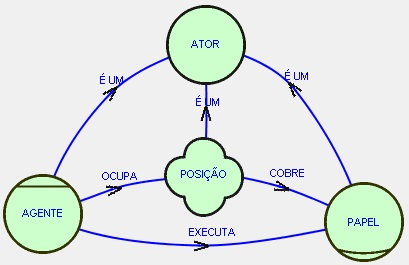
\includegraphics[scale=0.8]{Figuras/istar/atores.jpg}
                            \caption{Exemplo de relações entre atores \cite{santos2008istar}}
                            \label{fig:atores-exemplo}
                    \end{figure}

                    \begin{figure}[h!]
                        \centering
                            \subfigure[fig:ator:a][Ator]{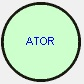
\includegraphics[scale=0.8]{Figuras/istar/ator.jpg}}
                            \subfigure[fig:ator:b][Agente]{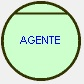
\includegraphics[scale=0.8]{Figuras/istar/ator-agente.jpg}}
                            \subfigure[fig:ator:c][Posição]{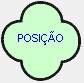
\includegraphics[scale=0.8]{Figuras/istar/ator-posicao.jpg}}
                            \subfigure[fig:ator:d][Papel]{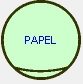
\includegraphics[scale=0.8]{Figuras/istar/ator-papel.jpg}}
                            \caption{Atores e especializações.}
                            \label{fig:atores}
                    \end{figure}
                    
                    %
                    \item \textbf{Agente} é a decomposição de um ator que possui manifestações físicas concretas. Refere-se tanto a humanos quanto a agentes de software ou hardware. Um agente possui dependências independentemente do papel que está executando. As características de um agente normalmente não são fáceis de se transferir para outros atores/agentes. São como experiências, habilidades ou, até mesmo, limitações físicas.
                    %
                    \item \textbf{Posição} representa uma abstração intermediária entre um agente e um papel. É o conjunto de papéis tipicamente executados por um agente, ou seja, representa uma posição dentro da organização onde o agente pode desempenhar várias funções (papéis). Diz-se que um agente ocupa uma posição e uma posição cobre um papel.
                    %
                    \item \textbf{Papel} é a caracterização abstrata do comportamento de um ator dentro de determinados contextos sociais ou domínio de informação. Essas características devem ser facilmente transferíveis a outro ator social. As dependências associadas a um papel são aplicáveis independentemente do agente que desempenha o papel.
                \end{enumerate}

            % actors associations
            \paragraph{Associações entre Atores:}
                As associações entre os atores são descritas através de links de associação (conforme a Figura \ref{fig:associations}.
                Essas associações podem ser de seis tipos:

                \begin{enumerate}[i.]
                    \item \textbf{\emph{IS PART OF}} (faz parte de) - Nessa associação cada papel, posição e agente pode ter sub-partes. Em \emph{IS PART OF} há dependências intencionais entre o todo e sua parte. Por exemplo, a dependência do todo sobre suas partes para manter a unidade na organização.

                    \item \textbf{\emph{ISA}} (é um) - Essa associação representa uma generalização, com um ator sendo um caso especializado de outro ator. Ambas, \emph{ISA} e \emph{IS PART OF}, podem ser aplicadas entre quaisquer duas instâncias do mesmo tipo de ator.
                    
                    \item \textbf{\emph{PLAYS}} (executa) - A associação plays é usada entre um agente e um papel, com um agente executando um papel. A identidade do agente que executa um papel não deverá ter efeito algum nas responsabilidades do papel ao qual está associado, e similarmente, aspectos de um agente deverão permanecer inalterados mesmo associados a um papel que este desempenha.
                    
                    \item \textbf{\emph{COVERS}} (cobre) - A associação covers é usada para descrever uma relação entre uma posição e os papéis que esta cobre.
                    
                    \item \textbf{\emph{OCCUPIES}} (ocupa) - Esta associação é usada para mostrar que um agente ocupa uma posição, ou seja, o ator executa todos os papéis que são cobertos pela posição que ele ocupa.
                    
                    \item \textbf{INS} - Esta associação é usada para representar uma \textbf{INS}tância específica de uma entidade mais geral. Por exemplo, quando se deseja representar um agente que é uma instanciação de outro agente.
                \end{enumerate}
                \begin{figure}[h!]
                    \centering
                        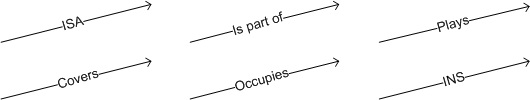
\includegraphics[width=0.8\linewidth]{Figuras/istar/actor-associations.jpg}
                        \caption{Tipos de associações entre atores \cite{site2013iwiki}.}
                        \label{fig:associations}
                \end{figure}

            % Elements
            \paragraph{Relação de Dependência}
                Uma relação de dependência pode ser deifinida como um acordo entre dois atores.
                Os elementos que compõe uma relação de dependência são:
                \begin{enumerate}[i.]
                    \item \emph{\textbf{Depender}}: é o ator dependente, ou seja, o ator que precisa que o acordo (\emph{Dependum}) seja realizado. Esse ator não se importa como o outro ator (\emph{Dependee}) irá satisfazer a necessidade da dependência.
                    \item \emph{\textbf{Dependum}}: é o elemento intermediário, objeto de questionamento e validação, da relação de dependência. % Ou seja, TODO
                    \item \emph{\textbf{Dependee}}: é o ator que tem a responsabilidade de satisfazer a relação de dependência.
                \end{enumerate}

                Dessa forma, pode-se classificar o tipo de uma relação de dependência com base em dos seguintes tipos de \emph{Dependum}:
                \begin{enumerate}[i.]
                    \item \textbf{Objetivo} (\emph{Goal}) - é uma declaração de afirmação sobre um certo estado do mundo. Deve ser de fácil verificação. O \emph{Dependee} é livre para tomar qualquer decisão para satisfazer o objetivo e é esperado que ele o faça. Não importa para o \emph{Depender} como o \emph{Dependee} irá alcançar esse objetivo.
                    %
                    \item \textbf{Tarefa} (\emph{Task}) - é uma atividade a ser realizada pelo \emph{Dependee}. Tarefas podem ser vistas com a realização de operações, processos e etc. Porém, não deve ser uma descrição passo-a-passo ou uma especificação completa de execução de uma rotina.
                    %
                    \item \textbf{Recurso} (\emph{Resource}) - é entidade (física ou informativa) a ser entregue para o \emph{Depender} pelo \emph{Dependee}. Satisfazendo-se esta dependência, o \emph{Depender} está habilitado a usar essa entidade como um recurso.
                    %
                    \item \textbf{Objetivo-Soft} (\emph{Softgoal}) - é semelhante ao Objetivo, porém os critérios de avaliação e verificação são mais subjetivos. O \emph{Depender} pode decidir sobre o que constitui a realização satisfatória do objetivo.
                \end{enumerate}
                % \begin{figure}[h!]
                %     \centering
                %         \includegraphics[width=0.7\linewidth]{Figuras/istar/dependency-links.jpg}
                %         \caption{Exemplo de Relação de Dependência (\emph{Dependder} -> \emph{Dependum} -> \emph{Dependee})}
                %         \label{fig:dependency-links}
                % \end{figure}
                % A Figura \ref{fig:dependency-links} apresenta alguns exemplos de relações de dependências.
            
            % Links (One side)
            \paragraph{Ligação de dependência}
                É uma estritamente a conexão entre os elementos de forma direcionada.
                Assim, pode-se ter somente duas opções de conexão: início no \emph{Depender}, fim no \emph{Dependum} e início no \emph{Dependum} e fim no \emph{Dependee}. Essa conexão é definida por um segmento contínuo, com a letra ``D'' sobrescrita, e direcionada da origem para o destino (conforme os exemplos da Figura \ref{fig:dependency}).
                % Assim, pode-se pensar na seguinte estrutura de nodos e ligações:
                %     1. \emph{Depender} (nodo); 2. Ligação de dependência (ligação); 3. \emph{Dependum} (nodo); 4. Ligação de dependência (ligação); 5. \emph{Dependee} (nodo).
                \begin{figure}[h!]
                    \centering
                        \subfigure[fig:dependency:empty][Ligação de Dependência.]{
\includegraphics[scale=1]{Figuras/istar/dependency-empty.jpg}}
                        \\
                        \subfigure[fig:dependency:depender-dependum][Ligação de Dependência: do \emph{Depender} para o \emph{Dependum}.]{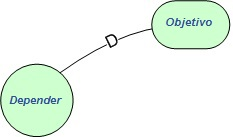
\includegraphics[width=0.4\linewidth]{Figuras/istar/dependency-depender-dependum.jpg}}
                        ~
                        \subfigure[fig:dependency:dependum-dependee][Ligação de Dependência: do \emph{Dependum} para o \emph{Dependee}.]{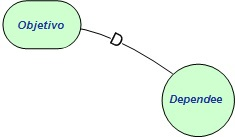
\includegraphics[width=0.4\linewidth]{Figuras/istar/dependency-dependum-dependee.jpg}}
                        \caption{Exemplos de ligação de dependência.}
                        \label{fig:dependency}
                \end{figure}
                
        % [end]
        \subsection{Modelos de Razões Estratégicas (SR)}
            % SR
                Já o modelo de Razões Estratégicas(SR)\footnote{SR, do inglês Strategic Rationale},
                representa os detalhes das razões internas que estão por trás das dependências dos atores.
                Com isso, é possível detalhar os interesses, preocupações e motivações específicas de um ator.
                Esse tipo de modelo também torna possível a avaliação de alteranativas em definições de processos.

                O modelo SR, além de poder conter todos os atores e dependências do SD, ``abre-se'' os Atores para se detalhar as dependências e expressar as razões.
                Ou seja, para os atores que precisam ser detalhados, é habilitado o limite da fronteira que deve estar visível e com espaço o suficiente para receber os elementos de dependência e/ou ligações internas. 
                Dessa forma, pode-se pensar nos elementos internos ao ator, ou seja, dentro da área de fronteira, como ``pertencentes'' ao ator.
                A seguir, são descritos os demais elementos de um modelo SR.

            \paragraph{Fronteira}
                Uma fronteira indica os limites intecionais de um determinado ator. Todos os elementos dentro dos limites de um ator, são explicitamente desejos ou pretenções desse ator. Uma fronteira é representada por um círculo tracejado e o elemento do ator dessa fronteira deve ser sobreposto a ela, ficando acima do tracejado (conforme a Figura \ref{fig:boundary}).

                \begin{figure}[h!]
                    \centering
                        \subfigure[fig:boundary:a][Fronteira Vazia]{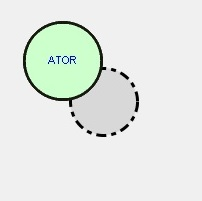
\includegraphics[width=0.3\linewidth]{Figuras/istar/boundary-empty.jpg}}
                        \subfigure[fig:boundary:b][Fronteira com elementos internos]{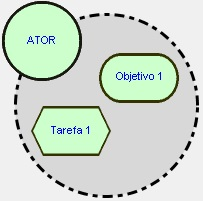
\includegraphics[width=0.3\linewidth]{Figuras/istar/boundary-non-empty.jpg}}
                        \caption{Exemplos de fronteira do ator.}
                        \label{fig:boundary}
                \end{figure}

            \paragraph{Ligação de meio-fim (\emph{means-end})}
                    % TODO: review.
                    É representada graficamente por uma seta direcionada ao nó fim, significando o meio para atingir um fim (objetivo, recurso, \emph{softgoal}, ou uma tarefa). A Figura \ref{fig:means-end} exemplifica este tipo de ligação.
                    \begin{figure}[h!]
                        \centering
                            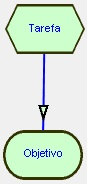
\includegraphics[scale=1]{Figuras/istar/means-end.jpg}
                            \caption{Exemplo de ligação meio-fim.}
                            \label{fig:means-end}
                    \end{figure}
                    %
                \paragraph{Ligação de decomposição (\emph{decomposition}):}
                    É responsável por detalhar e expressar da melhor como realizar uma determinada tarefa, através da decomposição em sub-elementos ligados  a  tarefa  principal (superior)  através  de  um  segmento  de  reta cortado.  Esses sub-elementos  podem  ser:  metas,  tarefas,  recursos  e  objetivos-soft.
                    \begin{figure}[h!]
                        \centering
                            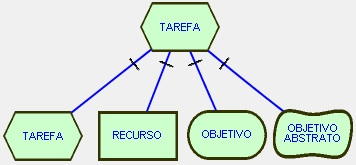
\includegraphics[scale=1]{Figuras/istar/decomposition.jpg}
                            \caption{Exemplo de ligação de decomposição.}
                            \label{fig:decomposition}
                    \end{figure}
                    %
                \paragraph{Ligações de Contribuição (\emph{contribution}):}
                    As ligações de contribuição são para ligar elementos à exclusivamente um objetivo-soft (\emph{softgoal}).
                    Essa ligação ajuda a modelar a forma como os elementos contribuem para a satisfação desse objetivo-soft (\emph{softgoal}).
                    Essas ligações de contribuição, ilustradas na Figura \ref{fig:contributions}, podem ser:
                    \begin{figure}[h!]
                        \centering
                            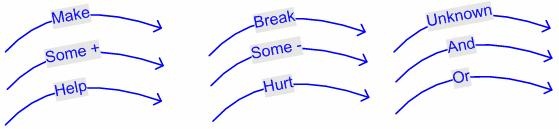
\includegraphics[scale=1]{Figuras/istar/contributions.jpg}
                            \caption{Ligações de contribuição \cite{site2013iwiki}.}
                            \label{fig:contributions}
                    \end{figure}
                    \begin{enumerate}[i.]
                        \item \textbf{\emph{Make}}: é uma contribuição positiva, suficientemente forte para satisfazer o objetivo-soft. 
                        \item \textbf{\emph{Some +}}: é uma contribuição positiva, mas cuja força de influência é desconhecida. Pode equivaler a um \emph{make} ou a um \emph{help}.
                        \item \textbf{\emph{Help}}: é uma contribuição positiva fraca, pois não é suficiente para que ela sozinha satisfaça o objetivo-soft.
                        \item \textbf{\emph{Unknown}}: é uma contribuição cuja influência é desconhecida. 
                        \item \textbf{\emph{Hurt}}: é uma contribuição negativa fraca, porém não é suficiente para que ela sozinha recuse a  satisfação de um objetivo-soft.
                        \item \textbf{\emph{Some -}}: é uma contribuição negativa, mas a força de sua influência é desconhecida. Pode equivaler a um \emph{hurt} ou a um \emph{break}.
                        \item \textbf{\emph{Break}}: é uma contribuição negativa, suficientemente forte para rejeitar a satisfação do objetivo-soft.
                        \item \textbf{\emph{Or}}: é uma contribuição onde o objetivo-soft é satisfeito se algum dos descendentes for satisfeitos. 
                        \item \textbf{\emph{And}}: é uma contribuição onde o objetivo-soft é satisfeito se todos os descendentes forem satisfeitos.
                    \end{enumerate}
                
        % [end]
        % \subsection{Diretrizes i* Wiki}
            %     % intro sobre as diretrizes
            %     No wiki do i* \cite{site2013iwiki} são apresentadas

            %     % TODO: reescrever
            %     As diretrizes são classificadas quanto ao nível:
            %         - iniciante: assume-se que o ?modelador? está tendo o primeiro contato com o framework de modelagem i*.
            %         - intermediário: 
            %         - avançado

            %     Quanto ao tipo:
            %         - conceito: esclarece questões sobre os fundamentos do framework
            %         - nomenclatura: como os atores, liks e elementos devem ser chamados? lida com questoes de cores e icones também.
            %         - notação: lida com a seleção adequada e uso da notação i* nos elementos, atores e links.
            %         - layout: lida com a disposição e organização dos modelos i* e o jeito que o conteúdo dos modelos 

        % [end]
    % [end]
    \section{Variações Baseadas no Framework i*}
        \label{cap:framework-sec:variacoes}
        % ITU-T = GRL + UCM.
        % yu95, i* wiki, GRL, Tropos, Aspectual i*, i*-c [6]
        % intro
            % Estudos da área já realizaram comparações entre as ferramentas.
            % Diferentes grupos de pesquisas que adotaram o framework i*.
            % Por vezes, o framework i* não atende todas as necessidades de um determinado grupo de pesquisadores.

        % exemplos
            % "O framework i* foi inicialmente proposto por [Yu 1995], mas hoje existem algumas extensões ou variações para sua versão original"
            % "Essas variações surgiram de diferentes grupos de pesquisa para atender ao propósito particular de cada um deles, e com isso surgiram diversas ferramentas de suporte."

        %problemas das variações i*
            % Conforme \cite{lucena2008}, as divergências quanto ao uso do i* podem causar:
            %     \begin{itemize}
            %         \item Divisão do esforço, ao passo que cada grupo de pesquisa irá focar no desenvolvimento de ferramentas de suporte ao seu próprio i*;
            %         \item Erros na semântica entre os projetistas e os leitores de um modelo particular do i*;
            %         \item Inibição da adoção/uso do i* por parte de novos usuários.
            %     \end{itemize}

        % vários estudos comparativos já foram realizados
            %http://istarwiki.org/tiki-index.php?page=i%2A+Modelling+Techniques&structure=i%2A+Wiki+Home
        % [end]
        \subsection{i* Wiki}
            % o que é?
                O i* Wiki, é um projeto criado com o intuito de reunir trabalhos relativos ao i*, de forma colaborativa
                    \cite{site2013iwiki} \cite{leuf2001wiki}.
                Com isso, a comunidade incentiva a colaboração dos usuários do framework, por meio de \emph{feedback} ou mesmo inserção de conteúdo em site oficial.
                Além disso, esses usuários podem sugerir alternativas ou extensões sintáticas e semânticas em relação a linguagem utilizada.
            
            % como funciona?
                Apesar da ampla visão que a comunidade pode ter com os trabalhos divulgados no site, a intenção é fornecer e evoluir uma única versão semântica do i*.
                Dessa forma, o i* Wiki funciona sobre duas versões do guia para o i* \cite{site2013iwiki}:
                    uma versão estável, servindo de referência para os usuários;
                    outra versão aberta a discussão, acessível aos usuários registrados no site e passível de comentários e sugestões individuais.
                Além disso, o site reúne um conjunto de Estudos de Casos, Publicações e Eventos relacionados a área de i*.
        % [end]

        \subsection{\emph{Goal-Oriented Requirements Language} (GRL)}
            A GRL é uma linguagem de apoio à modelagem orientada a agentes e objetivos.
            Assim como o i*, a GRL foca na modelagem dos relacionamentos estratégicos entre atores e seus objetivos.
            Pode-se pensar como uma alternativa que concentra recursos das metodologias NFR (\emph{Non-Functional Requirements}), i* e Tropos \cite{regev2005goals}.
            Outro ponto interessante é que a GRL é escalável, podendo se trabalhar com diferentes níveis de granularidade, em múltiplos diagramas ou visões de um mesmo modelo.

            Além disso, uma combinação da GRL com a \emph{Use Case Map} (UCM) deu origem a \emph{User Requirement Notation} (URN) - um padrão internacional do \emph{International  Telecommunication  Union} (ITU) para notação de requisitos de usuário.

        % [end]

        \subsection{Tropos}
            Tropos é um projeto que foi lançado em 2000 \cite{mylopoulos2001uml}, e visa apoiar a construção de sistemas de software orientados a agentes.
            O projeto reúne um grupo de autores de diversas Universidades no Brasil, Canadá, Bélgica, Alemanha, Itália, etc.
                % Tropos tem como objetivo o  desenvolvimento de sistemas de acordo com as reais necessidades de uma organização, buscando um melhor casamento entre o sistema e o ambiente em constante mudança.
            O processo de desenvolvimento segundo esta metodologia inicia com um estudo e elaboração de um modelo do ambiente no qual o sistema em desenvolvimento irá operar.
            Este modelo é refinado até que este represente o ambiente com o sistema em seu contexto.
            Cada modelo é descrito em termos dos atores observados no ambiente em modelagem, seus objetivos e relacionamentos.
            A metodologia Tropos oferece um framework que engloba as principais fases de desenvolvimento de software, com o apoio das seguintes atividades: Requisitos Iniciais, Requisitos Finais, Projeto Arquitetural e Projeto Detalhado.
        % [end]

    % [end]
    \section{Ferramenta OME }
        \label{cap:framework-sec:ferramentas}
        % intro
            Atualmente, existem várias ferramentas de modelagem i*.
            Pode-se encontrar mais de 20 ferramentas referenciadas no site do i* Wiki \cite{site2013iwiki}.
            % Ferramentas já foram comparadas. Listar trabalhos.
            Além disso, alguns trabalhos já realizaram comparações sobre ferramentas do framework i*,
                como em \cite{santos2008istar}(Tabela 6) e no site \cite{site2013iwiki}.

        % Pq só as duas?
            % Conforme foi comentado no Capítulo \ref{cap:introducao}, os arquivos de entrada aceitos pela JGOOSE devem estar no formato TELOS (.tel).
            % Além disso, conforme a apresentação da primeira versão da ferramenta em \cite{vicente2006}, as duas ferramentas que trabalham com esse formato são a OME e a OpenOME.
            % call next
            % Dessa forma, a OME e a OpenOME são apresentadas a seguir.

        % \subsection{OME}
            % intro
                O Ambiente de Modelagem Organizacional, tradução literal de OME - Organization Modelling Environment, é um editor gráfico de propósito geral para dar suporte à modelagem orientada a objetivo e/ou orientada a agentes.
                É uma aplicação Java para \emph{desktop} desenvolvida na Universidade de Toronto \cite{ome2013}.

            % about
                A ferramenta possui recursos que auxiliam o usuário no desenvolvimento e manipulação de modelos i* e NFR (\emph{Non-Functional Requirements}) \cite{chung2000non}.
                % history
                Em 2004, o desenvolvimento foi parado e seu código foi portado para a plataforma Eclipse \cite{eclipse}, dando origem a sua versão em código aberto chamda OpenOME \cite{horkoff2011openome}.
                % Aparentemente, a ferramenta parou na versão 3 (ou OME3) - mas ainda é mantida no site http://www.cs.toronto.edu/km/ome/.

                Apesar do seu desenvolvimento ter sido finalizado, ainda existem usuários da OME3.
                Além disso, a ferramenta possui um manual do usuário online (http://www.cs.toronto.edu/km/ome/docs/manual/manual.html) e é de fácil utilização. A maioria dos recursos i*, por exemplo, estão de acordo com \cite{yu1995modelling}.

            % exemplo final de tela:
                \begin{figure}[h!]
                    \centering
                        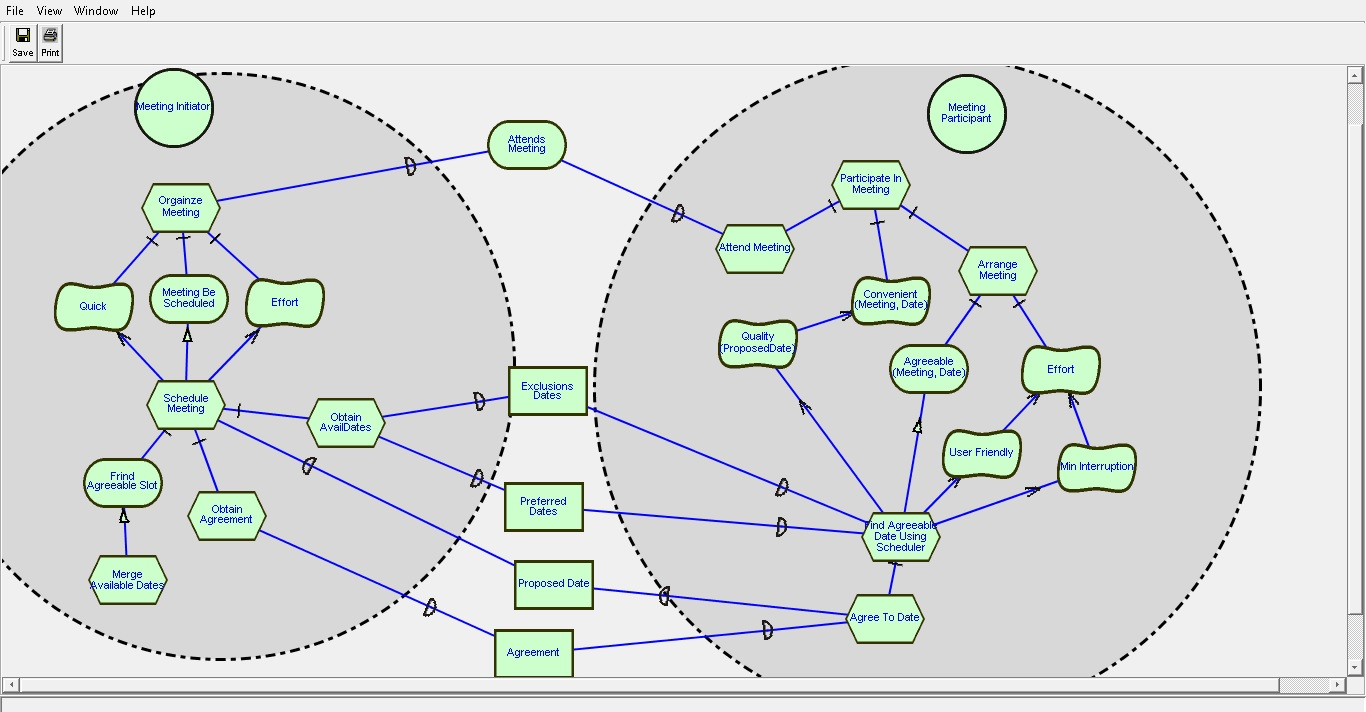
\includegraphics[width=0.8\linewidth]{Figuras/istar/tela-ome.jpg}
                        \caption{Exemplo de modelagem com a ferramenta OME3}
                        \label{fig:tela-ome}
                \end{figure}

                Como exemplo, têm-se na Figura \ref{fig:tela-ome} um dos modelos de exemplos já contidos na ferramenta OME3 junto à instalação (arquivo: ``Meeting-Schedule.tel'').
                Nessa tela, pode-se observar a barra de ferramentas (\emph{toolbar}) com as opções para criação dos elementos i*: atores, elementos de dependência, links  de  dependência, links  de  associação, etc.

                Cabe relembrar que essa ferramenta gera os modelos i* no formato TELOS, atualmente aceitos pela ferramenta JGOOSE.
                Além disso, considerando que a ferramenta apresenta problemas de instabilidade e seu processo de desenvolvimento foi descontinuado, acredita-se que a JGOOSE deva adotar uma nova solução para este fim.

    % [end]

    \section{iStarML}
        % intro
            Muitas ferramentas foram criadas com base nos conceitos do framework i* ou de variações desse \cite{cares2012towards} \cite{cares2011towards}.
            Isso acabou gerando modelos específicos para cada ferramenta, dificultando o intercâmbio de modelos entre essas ferramentas.
            Pensando nisso, foi desenvolvida a iStarML.
            Um meta-modelo baseado em XML (\emph{Extensible Markup Language}) usado para representar modelos i* \cite{cares2008istarml}.
            
            O principal objetivo desse meta-modelo é proporcionar um formato de intercâmbio entre os outros formatos de modelos do i*.
            Ou seja, a especificação iStarML deve suportar todas as outras definições e especificações dos modelos já propostos.
            Com isso, tudo o que se consegue especificar no formato TELOS, por exemplo, deve-se conseguir também no formato iStarML.

            Como prova de conceitos, foi realizado um estudo onde se aplicou o iStarML estritamente para fazer a interconexão entre duas ferramentas diferentes \cite{colomer2011model}.
            Nesse estudo, as ferramentas aplicadas foram jUCMNav \cite{kealey2006integrating} e a HiME \cite{lopez2009hime}.

            Porém, existe a preocupação sobre a real adoção da especificação iStarML. Como exemplo, tem-se a promessa da ferramenta OpenOME, que diz estar trabalhando para implementar rotinas de importação/exportação em iStarML \cite{horkoff2011openome} \cite{laue2011adding}.

            Conforme já mencionado no Capítulo \ref{cap:introducao}, é objetivo dessa pesquisa a implementação e adoção do iStarML como especificação do formato de arquivo padrão. Portanto, detalhes mais específicos sobre a linguagem iStarML serão feitas no Capítulo \ref{cap:proposta}.

    % [end]

    
    \section{Considerações Finais do Capítulo}
        \label{cap:framework-sec:conclusao}
        % o framework i* é importante (viu-se aplicações e benefícios em diversas áreas)
        %
            Neste Capítulo foram apresentados
                os conceitos gerais do framework i*, bem como as notaçãos da última versão do i* Wiki.
            Além disso,
                as variações do i* e seus respectivos meta-modelos, são estudados e analisados.
            Apesar das variações apresentadas, destaca-se a solução de intercâmbio entre diferentes formatos e ferramentas, iStarML.
            O iStarML foi adotado pelo editor proposto e será discutido melhor no Capítulo \ref{cap:proposta}.
    % [end]

% bibliography, just for auto-link in sublime text
% before compile main.tex, comment line below
% \bibliography{ref-unioeste,ref-commons,ref-books,ref-tecnologias,ref-istar}

% Capítulo 3
    \chapter{JGOOSE}
        \label{cap:jgoose}
        % intro
            Neste capítulo,
            é apresentada a ferramenta JGOOSE (\emph{Java Goal into Object Oriented Standard Extension}).
            %
            % Visão geral
            Inicialmente, na seção \ref{cap:jgoose-sec:overview},
                    % histórico
                    % diretrizes e passos
                são apresentados os principais conceitos, objetivos e as diretrizes que norteiam os processos de mapeamento de modelos organizacionais i* para casos de uso UML da ferramenta.
                Ainda nessa seção, também é apresentado um resumo histórico das versões ao longo dos anos e as principais contribuições de outros autores.
            % Projeto e Arquitetura
            Em seguida, na seção \ref{cap:jgoose-design},
                é analisada a organização estrutural da ferramenta, mostrando os impactos da proposta deste trabalho (\ferramenta{}) na estrutura e processos da JGOOSE.
        % [end]

    \section{Visão Geral}
        \label{cap:jgoose-sec:overview}
        % intro
            A JGOOSE é uma ferramenta de auxílio no mapeamento de modelos organizacionais para modelos funcionais \cite{vicente2006}.
            Essa ferramenta implementa seus processos guidados pelas diretrizes propostas por Santander \cite{santander2002integrando} e é com base nessas diretrizes que a ferramenta interpreta os modelos organizacionais do framework i* e gera os casos de uso UML, apresentando-os no \emph{template} proposto por Cockburn \cite{cockburn2001writing}.
            Com essa ferramenta, é possível derivar casos de uso com base nas intencionalidades associdadas aos atores de um ambiente organizacional.

            Na subseção a seguir, apresentaremos as diretrizes e passos da proposta de Santander \cite{santander2002integrando}, para posteriormente melhor compreender o funcionamento da ferramenta JGOOSE.
            E, na subseção seguinte (\ref{cap:jgoose-subsec:historico}), será apresentado um resumo histórico sobre as principais mudanças já ocorridas no projeto JGOOSE.

        \subsection{Diretrizes e Passos}
            O conjunto de diretrizes e passos propostos por Santander \cite{santander2002integrando} são a essência dos processos realizados pela ferramenta JGOOSE.
            É com base nessas diretrizes e passos que a ferramenta realiza o mapeamento de modelos organizacionais i* para modelos funcionais de Caso de Uso UML.
            A seguir, são descritas brevemente essas diretrizes e passos \cite{brischke2012melhorando}:

            \begin{enumerate}
                \item[1º Passo:] Descoberta de atores;
                \begin{enumerate}
                    \item[Diretriz 1:] todo ator em i* deve ser analisado sob um possível mapeamento para ator em caso de uso.
                    \item[Diretriz 2:] deve-se analisar se o ator em i* é externo ao sistema computacional pretendido, pois atores em caso de uso nunca são partes do sistema. Caso o ator seja externo ao sistema, o mesmo é considerado candidato a ator em Casos de Uso.
                    \item[Diretriz 3:] se o ator i* candidato tiver pelo menos uma dependência com o sistema computacional pretendido, esse deve ser um ator em caso de uso.
                    \item[Diretriz 4:] atores em i* relacionados através do mecanismo ISA, ou seja, com heranças de suas atividades nos modelos organizacionais e mapeados individualmente para atores em casos de uso (aplicando diretrizes 1, 2 e 3), serão relacionados no diagrama  de casos de uso através do relacionamento do tipo <<\emph{generalization}>>.
                \end{enumerate}

                \item[2º Passo:] Descoberta de Casos de Uso;
                \begin{enumerate}
                    \item[Diretriz 5:] para cada ator descoberto para o sistema no 1º passo, devemos observar todas as suas dependências (\emph{dependum}) como \emph{dependee} em relação ao ator que representa o sistema computacional pretendido (\emph{depender}), visando descobrir casos de uso para o ator.
                    \item[Subdiretriz 5.1:] deve-se analisar as dependências do tipo objetivo associadas com o ator e mapeadas diretamente para casos de uso.
                    \item[Subdiretriz 5.2:] deve-se avaliar as dependências do tipo tarefa associadas com o ator. Se um ator depende de outro ator para realizar uma tarefa, deve-se investigar se esta tarefa necessita ser refinada em subtarefas. Este tipo de tarefa pode ser mapeada para caso de uso.
                    \item[Subdiretriz 5.3:] deve-se avaliar as dependências do tipo recurso associadas com o ator. Se um ator depende de outro ator para obter um recurso, por que o mesmo é requerido? Se para esta resposta existe um objetivo, o mesmo será candidato a ser um objetivo de um caso de uso para este ator.
                    \item[Subdiretriz 5.4:] deve-se avaliar as dependências do tipo objetivo-soft associadas com o ator. Normalmente uma dependência do tipo objetivo-soft em i* é um requisito não-funcional associado ao sistema pretendido.
                    \item[Diretriz 6:] analisar a situação especial na qual um ator de sistema (descoberto seguindo as diretrizes do passo 1) possui dependências (como \emph{depender}) em relação ao ator em i* que representa o sistema computacional pretendido ou parte dele (ator $\rightarrow$ \emph{dependum} $\rightarrow$ sistema computacional).
                    \item[Diretriz 7:]  classificar cada caso de uso de acordo com seu tipo de objetivo associado: contextual, de usuário ou de subfunção.
                \end{enumerate}

                % \item[3º Passo:] Descoberta e descrição do fluxo principal e alternativo dos Casos de Uso.
                \item[3º Passo:] Especificação de Caso de Uso;
                \begin{enumerate}
                    \item[Diretriz 8:] analisar cada ator e seus relacionamentos no modelo de Razões Estratégicas (SR) para extrair informações que possam conduzir à descrição de fluxos principais e alternativos, bem como, pré-condições e pós-condições dos casos de uso descobertos para o ator.
                    %
                    Para isso precisamos analisar os subcomponentes em uma ligação de decomposição de tarefa mapeando-os para passos na descrição do cenário primário (fluxo principal) de casos de uso.
                    %
                    Também devemos analisar ligações do tipo meio-fim mapeando os meios para passos alternativos na descrição de casos de uso.
                    %
                    \item[Diretriz 9:] investigar a possibilidade de derivar novos objetivos de casos de uso a partir da observação dos passos nos cenários (fluxos de eventos) dos casos de uso descobertos.
                    %
                    \item[Diretriz 10:] Desenvolver o diagrama de casos de uso utilizando os casos de uso descobertos e os relacionamentos do tipo <<\emph{include}>>, <<\emph{extend}>> e <<\emph{generalization}>> usados para estruturar as especificações dos casos de uso.
                \end{enumerate}
            \end{enumerate}
        %

        \subsection{Resumo Histórico}
            \label{cap:jgoose-subsec:historico}
            % intro
                Desde a sua primeira versão \cite{vicente2006}, a ferramenta JGOOSE passou por várias melhorias e aprimoramentos.
                Mudanças essas que variam desde a refatoração de código fonte (Classes e \emph{Packages} Java) até alterações na interface gráfica do usuário \cite{brischke2011melhorando}.
                A seguir, é apresentado um resumo sobre a origem da JGOOSE e as principais alterações já realizadas na ferramenta.
            % 
            \begin{itemize}
                \item \textbf{GOOSE} -
                    % Marcelo Brischke
                    A \emph{Goal into Object Oriented Standard Extension} (GOOSE), foi a ferramenta que antecedeu à JGOOSE.
                        Implementada com a linguagem de programação \emph{Object Pascal} e com a extensão \emph{Rational Rose} por Marcelo Brischke \cite{brischke2005desenvolvimento}, possuía dependências das ferramentas OME e Rational Rose.
                    Devido a dependência dessa última, que é uma solução proprietária, a GOOSE foi distribuída sob uma licença educacional.
                    Analisando sob aspectos técnicos e funcionais, a ferramenta não contemplava todas as diretrizes propostas por Santander \cite{santander2002integrando}. Mais especificamente, as diretrizes 5.7, 7 e 9 não eram satisfeitas pelo processo do sistema \cite{brischke2005desenvolvimento}.

                \item \textbf{JGOOSE versão 2006} -
                    % André Abe Vicente
                    Desenvolvida por André Abe Vicente \cite{vicente2006},
                        a nova implementação passou a ser na linguagem Java e, com isso, foi atribuído o nome de JGOOSE (\emph{Java Goal into Object Oriented Standard Extension}).
                    Por ser em uma nova linguagem de programação, todo o projeto teve que ser re-implementado em Java.
                    Entre outros aspectos, a solução continuou dependente da ferramenta OME, contudo não utilizava mais a extensão Rational Rose.
                    Além disso, essa versão contou com a implementação da subdiretriz 5.4, aperfeiçoamento de outras subdiretrizes e novas funcionalidades de auxílio ao usuário no processo de mapeamento \cite{vicente2006}.

                \item \textbf{JGOOSE versão 2011} -
                    % Mauro Brischke
                    Melhorada por Mauro Brischke \cite{brischke2011melhorando},
                        a nova versão contempla a implementação de três diretrizes faltantes: 8, 9 e 10.
                    Também foi fruto desse trabalho a implementação da exportação dos casos de uso no formato XMI, melhorando a comunicação com outras ferramentas como a StarUML.
                    Nessa versão, foi implementado soluções que permitiram o usuário da ferramenta a realizar um refinamento manual dos casos de uso gerados, bem como visualizar graficamente os casos de uso na forma de imagens estáticas.

                \item \textbf{JGOOSE versão 2013} - 
                    Essa versão está em fase de desenvolvimento por Diego Peliser \cite{peliser2013aprimorando} e visa a correção de alguns \emph{bugs} na aplicação das diretrizes e a otimizações de código (algoritmos), bem como melhorias na interface gráfica e na documentação.
            \end{itemize}

        % finalizacao comparativa? - Com base nesse resumo histórico...
    % [end]

    \section{Projeto e Arquitetura}
        \label{cap:jgoose-design}
            Conforme o resumo histórico, a JGOOSE sofreu várias alterações ao longo dos anos.
            Entretanto, nenhuma dessas alterações influenciaram de forma significativa o fluxo de dados tradicional da ferramenta, mantendo como base as diretrizes e passos propostos por Santander \cite{santander2002integrando}.
            A figura \ref{fig:jgoose-arquitetura} foi apresentada por Brischke \cite{brischke2011melhorando} como sendo a represetanção da arquitetura da ferramenta JGOOSE.

            \begin{figure}[h!]
                \centering
                    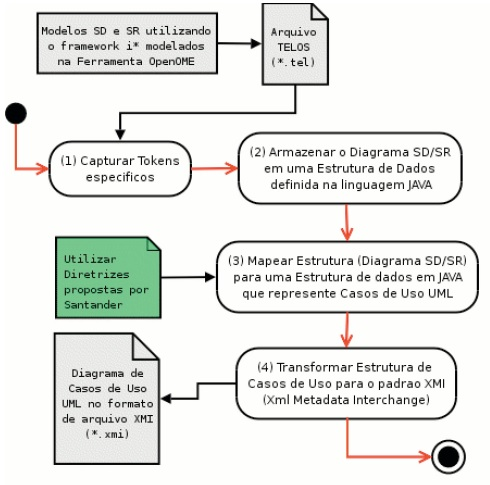
\includegraphics[scale=1]{Figuras/jgoose-arquitetura.jpg}
                    \caption{Figura apresentada por Brischke como ``Arquitetura da ferramenta JGOOSE Demonstrando o seu Funcionamento'' \cite{brischke2011melhorando}.}
                    \label{fig:jgoose-arquitetura}
            \end{figure}

            A figura \ref{fig:jgoose-arquitetura} foi analisada e refeita sobre os conceitos de DFD (\emph{Data Flow Diagram}) nos modelos de Gane e Sarson \cite{gane1977structured}.
            Antes de apresentar o novo diagrama sobre o fluxo de dados da JGOOSE, precisamos entender os elementos do DFD usados nesse diagrama.
            
            Nesse tipo de modelo (DFD), temos os seguintes elementos (apresentados na figura \ref{fig:dfd-captions}):

            % def. elementos DFD
                \begin{figure}[h!]
                    \centering
                        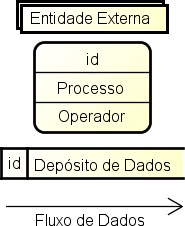
\includegraphics[scale=0.8]{Figuras/dfd-captions.png}
                        \caption{Elementos da notação Gane e Sarson \cite{gane1977structured} de DFD.}
                        \label{fig:dfd-captions}
                \end{figure}

                \begin{itemize}
                    \item \textbf{Entidade Externa}
                        - representam elementos de fora do sistema, mas que comunicam-se com ele.
                        São fontes de entradas de dados para o sistema ou destinos para as saída dos dados e contém apenas o \emph{nome} da entidade na sua representação.
                    %
                    \item \textbf{Processo} 
                        - representa uma transformação dos dados de entrada em dados de saída.
                        Contém um \emph{id}entificador único, um \emph{nome} do processo e o \emph{operador} do processo.
                    %
                    \item \textbf{Depósito de Dados}
                        - representa um repositório de dados no sistema, podendo ser tanto em banco de dados quanto em arquivos.
                        Contém um \emph{id}entificador único e o \emph{nome} do depósito de dados.
                    %
                    \item \textbf{Fluxo de Dados}
                        - representam canais através do qual passam as informações. Aplica-se uma etiqueta para representar os dados que ``passam'' por esse canal.
                \end{itemize}

            % diagrama de contexto
                Em modelos de DFD, existem os chamados \emph{diagramas de contexto DFD}, que expressam, em mais alto nível de abstração, a interação entre \emph{entidades externas} e somente um \emph{processo} do sistema \cite{gane1977structured}. Esse único processo deve resumir e representar as funções principais do sistema.
                Com base nesses conceitos,
                    foi construído um diagrama de contexto DFD (figura \ref{fig:dfd-context}) para representar o fluxo de dados entre a \emph{entidade externa} OME3, o \emph{processo} realizado pelo \emph{operador} JGOOSE e a \emph{entidade externa} StarUML.
                
                    \begin{figure}[h!]
                        \centering
                            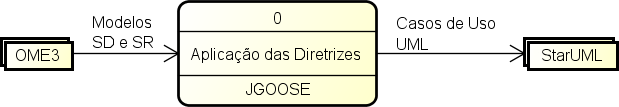
\includegraphics[scale=0.8]{Figuras/dfd-context-3.png}
                            \caption{Diagrama de contexto da Ferramenta JGOOSE.}
                            \label{fig:dfd-context}
                    \end{figure}

            % diagrama DFD
            Para melhor representar o fluxo de dados da JGOOSE, um diagrama com maiores detalhes nos processos foi construído e apresentados na figura \ref{fig:dfd-detail-1}.
            Esse diagrama visa representar a ``antiga estrutura'' da figura \ref{fig:jgoose-arquitetura} na forma de DFD tradicional, mostrando a \emph{entidade externa} OME3, os \emph{processos} da atual JGOOSE e \emph{entidade externa} StarUML.

            \begin{figure}[h!]
                \centering
                    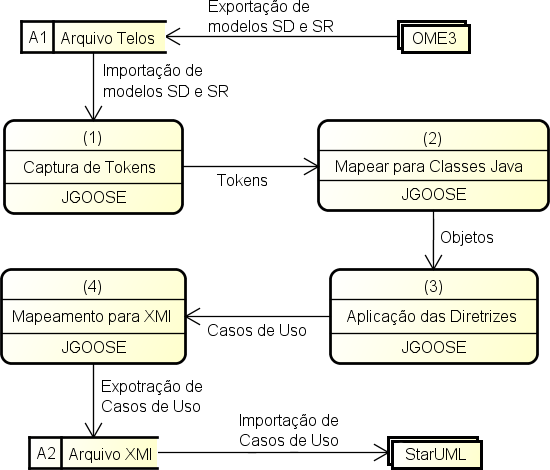
\includegraphics[scale=0.8]{Figuras/dfd-detail-1.png}
                    \caption{Diagrama de Fluxo de Dados da Ferramenta JGOOSE.}
                    \label{fig:dfd-detail-1}
            \end{figure}

        \subsection{Impacto da \ferramenta{}}
            Para realizar a integração da \ferramenta{} com a JGOOSE, serão necessárias algumas modificações do fluxo de dados original da JGOOSE.
            Conforme a proposta deste trabalho, que trata da manipulação de diagramas SD e SR,
                os processos ``(1) - Captura de Tokens - JGOOSE'' e ``(2) - Mapear para Classes Java - JGOOSE''
                deverão ser gerenciados pela \ferramenta{}.
                Dessa forma, um novo diagrama de fluxo de dados com a \ferramenta{}, é apresentado a seguir (figura \ref{fig:dfd-proposta}):
                \begin{figure}[h!]
                    \centering
                        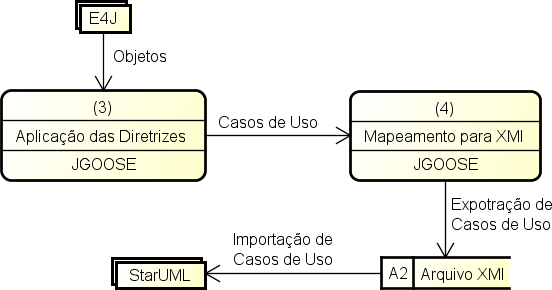
\includegraphics[scale=0.8]{Figuras/dfd-proposta.png}
                        \caption{Novo DFD da ferramenta JGOOSE, após integração com \ferramenta{}.}
                        \label{fig:dfd-proposta}
                \end{figure}

            Após a integração entre as duas ferramentas, não será mais possível executar diretamente a JGOOSE, pois essa passa a ser um módulo interno da \ferramenta{} (mais detalhes dessa integração serão apresentados na seção \ref{cap:proposta-sec:maven} do capítulo \ref{cap:proposta}).
            O processo de mapeamento se iniciará dentro da \ferramenta{} e, após as rotinas de mapeamento da estrutura em iStarML para a estrutura legada da JGOOSE, a linha de execução do programa passa a ser de responsabilidade da JGOOSE.
            Somente após o fechamento da interface da JGOOSE é que a linha de execução retorna ao gerenciamento da \ferramenta{}.

            Com isso, um novo diagrama de contexto DFD, onde a \ferramenta{} passa a ser o processo principal, é apresentada na figura \ref{fig:dfd-context-e4j}.
                \begin{figure}[h!]
                    \centering
                        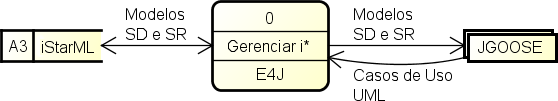
\includegraphics[scale=0.8]{Figuras/dfd-context-e4j.png}
                        \caption{Novo diagrama de contexto com a \ferramenta{} sendo o processo principal.}
                        \label{fig:dfd-context-e4j}
                \end{figure}
    % [end]

    \section{Considerações Finais do Capítulo}
        Considerando os processos que serão de responsabilidade da \ferramenta{},
            é conveniente pensar na incorporação da JGOOSE à \ferramenta{}, pois é com a \ferramenta{} que se inciam os processos que antecedem o mapeamento da JGOOSE.
        Dessa forma, a JGOOSE passará a cuidar especificamente das rotinas (diretrizes e passos) de mapeamento da estrutura (objetos e classes) i* para a estrutura de casos de uso UML, enquanto a \ferramenta{} trata dos processos iniciais de manipulação dos diagramas organizacionais.
        Em trabalhos futuros, pode-se estudar a viabilidade da alteração de algumas estruturas e rotinas da JGOOSE para usar as mesmas estruturas (objetos e classes) que a \ferramenta{}.
        Vale ressaltar que a integração \textbf{não afetará} a forma com a qual a JGOOSE realiza suas funções de mapeamento. Apenas deixará de executar suas rotinas de interpretação dos modelos organizacionais feitos em TELOS.
    % [end]

% bibliography, just for auto-link in sublime text
% before compile main.tex, comment line below
% \bibliography{../referencias/unioeste,../referencias/commons,../referencias/books,../referencias/tecnologias,../referencias/istar}

\chapter{Proposta}
    \label{cap:proposta}
    % intro
        % Neste capítulo, ...
    % retoma a "chamada" do Cap 1 ?!

    \section{Visão Geral}
        \label{cap:proposta-sec:overview}
        % tópico - intro
        \subsection{Conceitos e Considerações Iniciais}
            % tópico
    \section{Projeto e Arquitetura}
        \label{cap:proposta-sec:design}
        % tópico - intro
        \subsection{Modelagem i*}
            % será usado no projeto de IC
            % fazer a modelagem em um software qualquer (OpenOME ou OME)
            % refazer ele no estudo de caso?
            % Modelos SD e SR
            % Use Case Gerado...
        \subsection{Arquitetura Modular}
            % tópico
            % reuso de software: Ivonei
            % linhas de produção: Ivonei
        \subsection{Maven}
            % o que é?
            % como funciona?
            % como usei?
            % que resultados obtive
            % o que esperar?
    %
    \section{Desenvolvimento}
        \label{cap:proposta-sec:development}
        % tópico - intro
            % introdução
                % conexão com o tópico anterior
                % problemas
                    % atuais
                    % comuns
                    % referências de trabalhos recentes
                % importância do tópico
                % conceitos importantes
                    % referências "Clássicas"
            % desenvolvimento
                % relação do tópico com o trabalho geral
                % relação do tópico com outro tópico?
                % outros trabalhos que já fizeram "essa conexão"
            % fechamento ou conexão para o tópico seguinte
        %\subsection{}
            % tópico
    %
    \section{Recursos}
        % tópico
        \subsection{Internacionalização (i18n)}
            % o que é?
            % pq é importante?
            % como foi feito?
            % outros pontos importantes?
            % usa padrões de projeto?
        \subsection{UndoManager}
        % \subsection{TODO}
        \subsection{API iStarML}
    \section{Testes e Validação}
        % tópico - intro
            % introdução
                % conexão com o tópico anterior
                % problemas
                    % atuais
                    % comuns
                    % referências de trabalhos recentes
                % importância do tópico
                % conceitos importantes
                    % referências "Clássicas"
            % desenvolvimento
                % relação do tópico com o trabalho geral
                % relação do tópico com outro tópico?
                % outros trabalhos que já fizeram "essa conexão"
            % fechamento ou conexão para o tópico seguinte
        \subsection{Testes Unitários}
            % tópico
                % introdução
                    % conexão com o tópico anterior
                    % problemas
                        % atuais
                        % comuns
                        % referências de trabalhos recentes
                    % importância do tópico
                    % conceitos importantes
                        % referências "Clássicas"
                % desenvolvimento
                    % relação do tópico com o trabalho geral
                    % relação do tópico com outro tópico?
                    % outros trabalhos que já fizeram "essa conexão"
                % fechamento ou conexão para o tópico seguinte
    \section{Considerações Finais do Capítulo}

% Não pode ser usado o termo 'estudo de caso' para este capítulo!
% "Exemplos de Uso" é igual ao capítulo 5 da Dissertação da Bárbara. (IStarTool)
\chapter{Exemplos de Uso}
    \label{cap:estudo-de-caso}
        % retoma a "chamada" do Cap 1 ?!
        % intro
            % Neste capítulo, ...
        % Qual o tipo de Estudo de Caso? (ver recomendações do Victor) e explicitar no cap 1 !!!
        % Como foi aplicado esse tipo de EC

    \section{Pré-requisitos e Instalação do Sistema}
        % Como instalar?
        % O que é preciso para instalar?

    \section{Conhecendo a Ferramenta}
        % Manual, Telas Numerada, Passo a Passo, etc.

    \section{Usando a Ferramenta}
        % Intro
            % descrever um exemplo! (o próprio TCC?)
        Para fins de exemplo de uso da ferramenta,
            será desenvolvido o mesmo modelo organizacional feito no capítulo anterior - agora com a E4J.

        \subsection{Modelos SD e SR}
            % Desenvolver SD e SR - igual ao cap anterior

        \subsection{Exportando para iStarML}
            % Exportar iStarML e mostrar o resultado arquivo XML

        \subsection{Gerando Casos de Uso com a JGOOSE}
            % Do-it! Saiu igual ao capítulo anterior?

    \section{Resultados e Análises}
        % saiu conforme o esperado?
        % a ferramenta se comportou bem? hehe

    \section{Considerações Finais do Capítulo}

%\chapter{Resultados e An\'{a}lises}
...

% Conclusão
    \chapter{Considerações Finais}
        \label{cap:conclusao}
        % intro
            % Neste capítulo, ...
        % retoma a "chamada" do Cap 1 ?!
    % atingiu os objetivos? ->
        % sim, em tudo
        % sim, parcialmente. mostrar os motivos
        % não. pq? mostrar os motivos
    \section{Contribuições}
        % publicou ou vai publicar?
    \section{Trabalhos Futuros}
        % intro
        % \subsection{}
            % intro



% Inclusão dos apêndices
\oneandhalfspacing
\appendix
\chapter{iStarML API}
\label{apendice:istarml}

\section{Introdu\c{c}\~{a}o}
...

\section{Projeto e Arquitetura}
...

\section{Documenta\c{c}\~{a}o}
...

% Inclusão dos anexos
% \chapter{Guia i*}
\label{anexo:guia}
intro...
origem e justificativa..
sobre a estrutura do guia...
...
o guia 

% incluindo o glossário
% \chapter*{Gloss\'{a}rio}
\addcontentsline{toc}{chapter}{Gloss\'{a}rio}

\begin{tabular}{ll}
Stakeholders &  S\~{a}o todos os envolvidos, pessoas ou organiza\c{c}\~{o}es, que ser\~{a}o afetadas pelo\\
             &  sistema e que possuem influ\^{e}ncia, direta ou indireta, sobre os requisitos
\end{tabular}

% \pagebreak

% Referências Bibliográficas
% \bibliographystyle{abnt-alf}
\bibliographystyle{abnt-num} % use 'abnt-num.bst'
\pagebreak
\addcontentsline{toc}{chapter}{Referências Bibliográficas}

% \citeoption{abnt-etal-cite=2} % only abnt-alf
\bibliography{referencias/abnt-options,referencias/_example,referencias/unioeste,referencias/commons,referencias/books,referencias/tecnologias,referencias/istar}

\end {document}	%% Fim do Documento
